\chapter{Implementation}
We implemented the Computer system in OMNeT++.\\
Figure \autoref{fig:omnetpp_implementation} provides an overview of the system implementation. Below is a detailed explanation of each module:
\begin{itemize}
    \item \texttt{ProcessGenerator}: this module generates processes according to a specified interarrival time distribution. Each process is assigned a total duration $D$, and the duration of each phase (initial, I/O, and final) is set to $0.4 D$, $0.2 D$, and $0.4 D$ if the process is CPU bound, or $0.1 D$, $0.8 D$, and $0.1 D$ if the process is I/O bound. The process is then sent to the scheduler.
    \item \texttt{scheduler}: this module contains an infinite-capacity queue. If \texttt{isFCFS} is set to \texttt{true}, a FIFO queue is used. Otherwise, a priority queue is used, with processes ordered by increasing duration until the I/O phase or termination (shortest job first).\\
    When the scheduler receives a process, it sends it to the first free CPU. If no CPU is free, the process is enqueued. When a CPU is freed, the next process in the queue is sent.
    When a process enters the I/O phase, the scheduler waits for the specified I/O phase duration and adds the process back into the queue.
    \item \texttt{cpu}: There are $N$ CPUs which operate independently. Each one, when it is free, receives a process from the scheduler and simulates its execution. When it finishes the execution phase (i.e. the I/O phase is reached or the process terminates), a message is sent to the scheduler, indicating that the CPU is now free.
\end{itemize}

\begin{figure}[H]
    \captionsetup{type=figure}
    \centering
    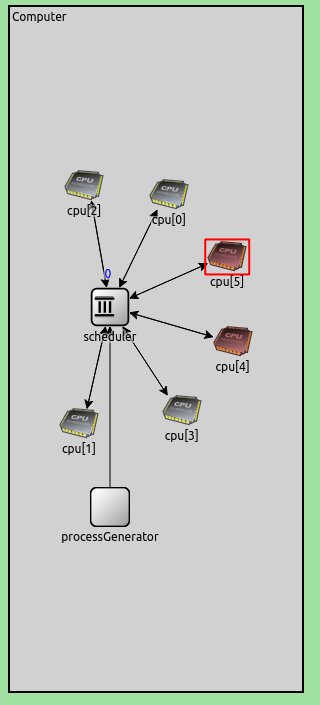
\includegraphics[width=0.4\textwidth]{images/example/sim_schema.png}
    \captionof{figure}{View of the system implementation in OMNeT++}
    \label{fig:omnetpp_implementation}
\end{figure}

